\subsubsection*{Tilpasning af træningsniveau} \label{sec:traeningsniveau}
Træningen tilgås fra hovedmenuen, dog skal træningsniveauet tilpasses brugeren førend træningen kan påbegyndes. Tilpasning af træningsniveau er en funktionalitet, der skal tage højde for daglige variationer ved at anbefale et træningsniveau ud fra brugeres kategorisering, daglig helbredstilstand og tidligere evaluering.  
Aktivitetsdiagrammet over tilpasning af træningsniveau fremgår af \autoref{fig:traeningsniveau}.

\begin{figure} [H]
\centering
\textbf{Aktivitetsdiagram: Tilpasning af træning}\par\medskip
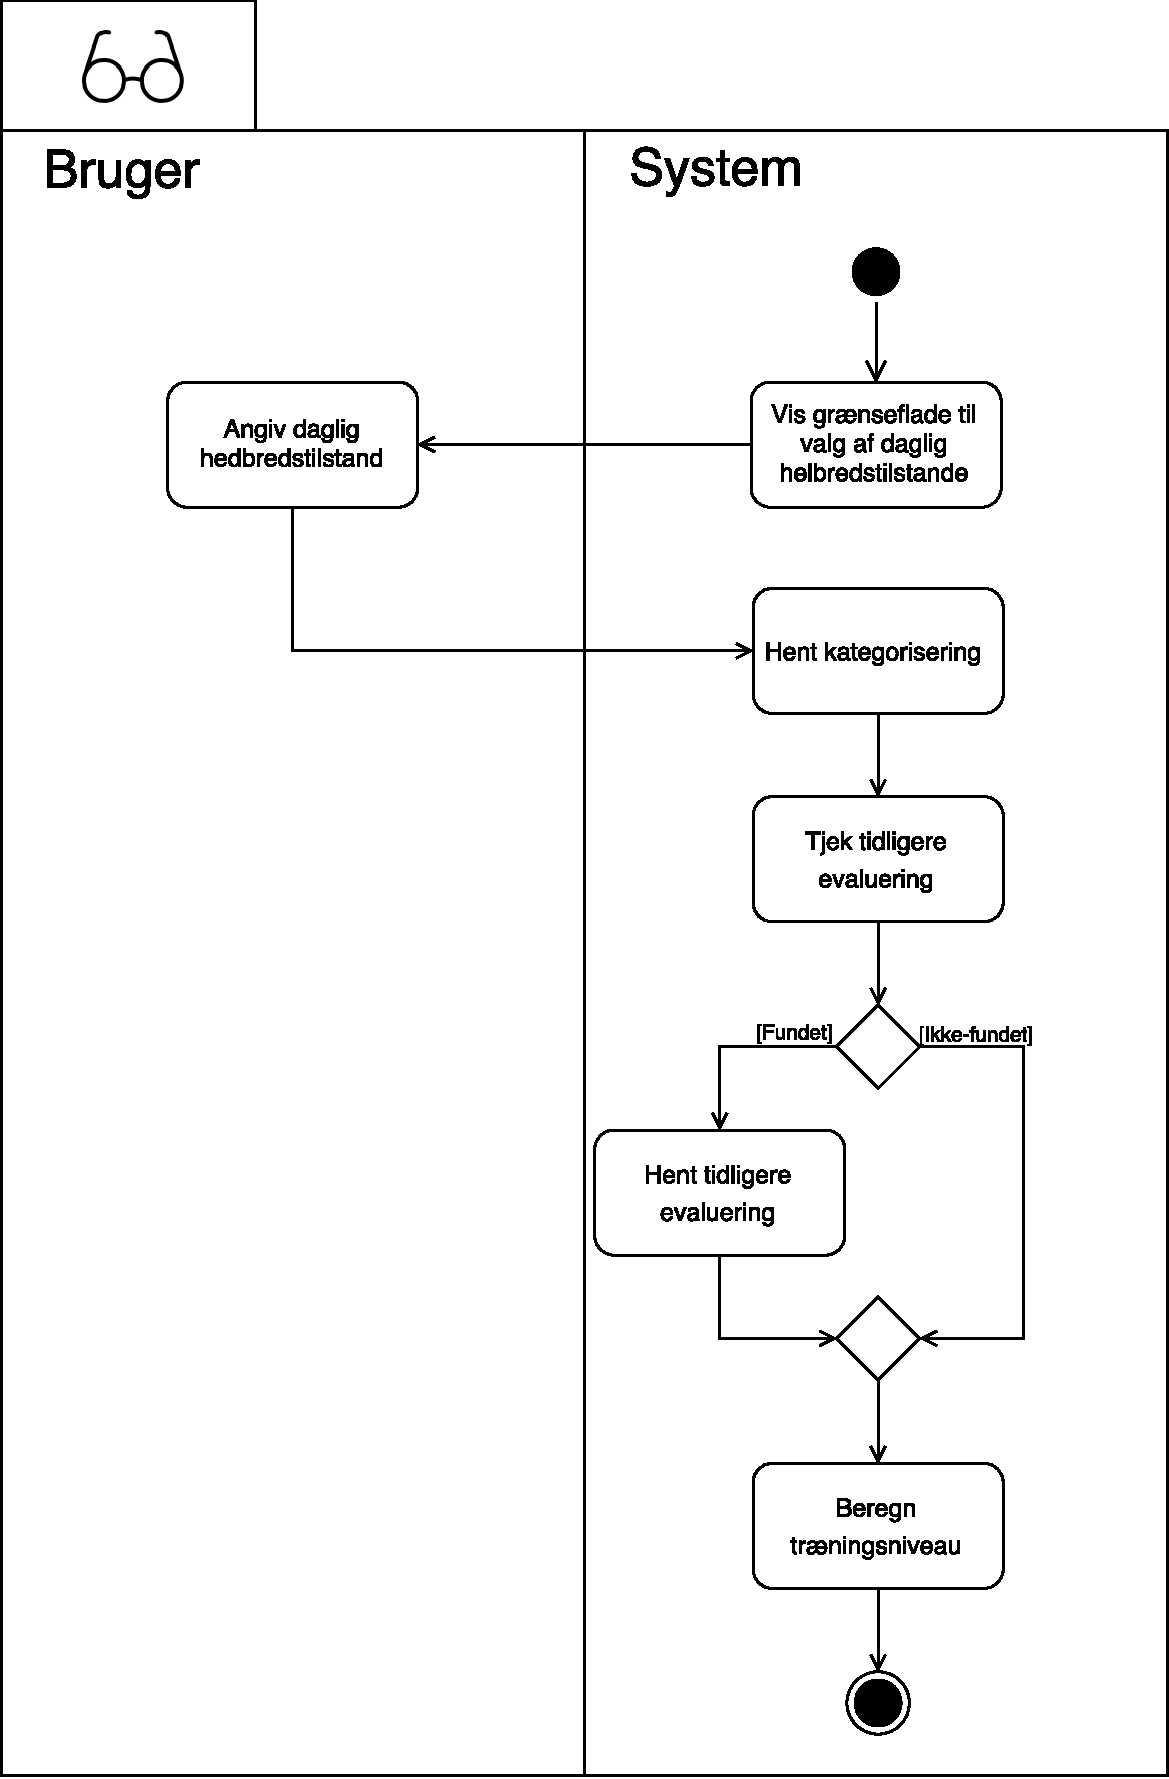
\includegraphics[width=0.9\textwidth]{figures/aktivitetsdiagram/Tilpasningaftraeningsniveau}
\caption{Aktivitetsdiagram over tilpasning af træningsniveau.}
\label{fig:traeningsniveau}
\end{figure}

\noindent
Systemet viser grænsefladen for valg af træningsform, hvor brugeren skal angive den ønskede træningsform, herunder konditions-, styrketræning eller vejrtrækningsøvelser. Ud fra den valgte træningsform skal brugeren angive træningstype, eksempelvis kan der ved valg af konditionstræning vælges gå, løbe eller cykle. Herefter vises grænsefladen for valg af daglige helbredstilstande, hvortil brugeren skal angive sin helbredstilstand. Systemet henter kategorisering fra brugeroplysninger, som oprettes i forbindelse med log ind, hvorefter den anmoder om tidligere evaluering i databasen. Databasen validerer, om der er en tidligere evaluering passende til træningen samt helbredstilstanden. Hvis brugeren ikke har angivet tidligere evaluering, bestemmes niveauet ud fra de resterende parametre. Hvis der findes en tidligere evaluering hentes denne og medregnes som en parameter. Et simpelt eksempel på denne beregning fremgår af \autoref{tab:beslutningstabel}. Tabellen beskriver, hvordan en algoritme vil kunne regulere træningsniveauet, således der tages højde for den enkelte bruger.

\begin{table}[H]
\centering
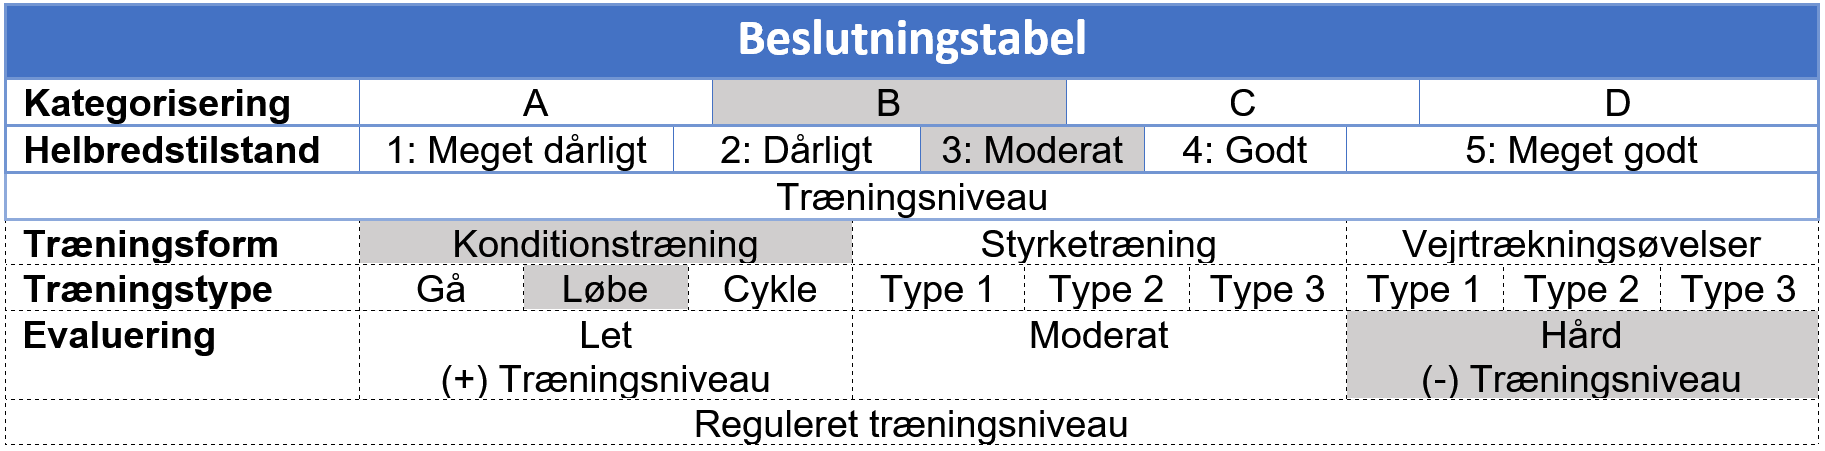
\includegraphics[width=1\textwidth]{figures/aktivitetsdiagram/beslutningstabel}
\caption{En simpel beslutningstabel for tilpasning af træningsniveau uden tidligere evaluering.}
\label{tab:beslutningstabel}
\end{table} 

\noindent
Af \autoref{tab:beslutningstabel} fremgår en simpel beslutningstabel for, hvorledes et træningsniveau tilpasses den enkelte bruger. Beslutningstabellen tager udgangspunkt i brugerens kategorisering, valgt træningsform og -type samt daglig helbredstilstand. Brugeren er i dette tilfælde kategoriseret til B, og har valgt at udføre konditionstræning herunder løb. Helbredstilstanden angives førend en træning påbegyndes, for således at tilpasse niveauet til den pågældende dag. Helbredstilstanden angives fra 1 til 5, hvortil brugerens helbredstilstand i dette eksempel angives som 3. Den simpel beslutningstabel udvælger dertil et træningsniveau. Dette træningsniveau kan yderligere tilpasses, hvis en passende evaluering tidligere er foretaget. En simpel beslutningstabel for dette, fremgår af \autoref{tab:beslutningstabel1}.

\begin{table}[H]
\centering
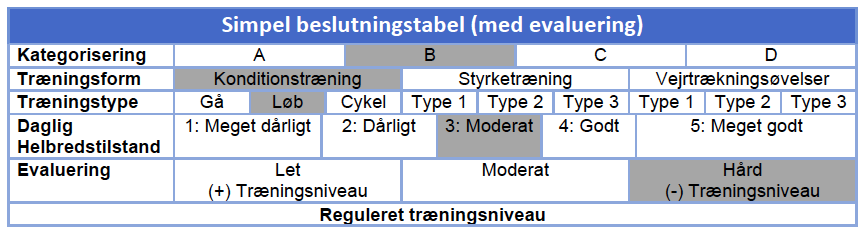
\includegraphics[width=1\textwidth]{figures/aktivitetsdiagram/beslutningstabel1}
\caption{En simpel beslutningstabel for tilpasning af træningsniveau med tidligere evaluering.}
\label{tab:beslutningstabel1}
\end{table} 

\noindent
Er en tidligere evaluering baseret på samme træningsform, -type samt helbredstilstand, kan træningen tilpasses denne. Af \autoref{tab:beslutningstabel1} fremgår en simpel beslutningstabel med evaluering. Brugeren har hertil samme kategorisering, træningsform samt -type, helbredstilstand som i eksemplet fra \autoref{tab:beslutningstabel1}. Dog er der hertil angivet en tidligere evaluering som værende hård. Dette medvirker til, at algoritmen regulerer træningsniveauet for denne træning, for således at give brugeren en bedre og mere tilpasset træningsoplevelse.


\subsection*{Træning} \label{sec:traening}
Efter tilpasning af træningsniveauet kan brugeren påbegynde en træning. Aktivitetsdiagrammet over træningen fremgår af \autoref{fig:traening}. 

\begin{figure} [H]
\centering
\textbf{Aktivitetsdiagram: Træning}\par\medskip
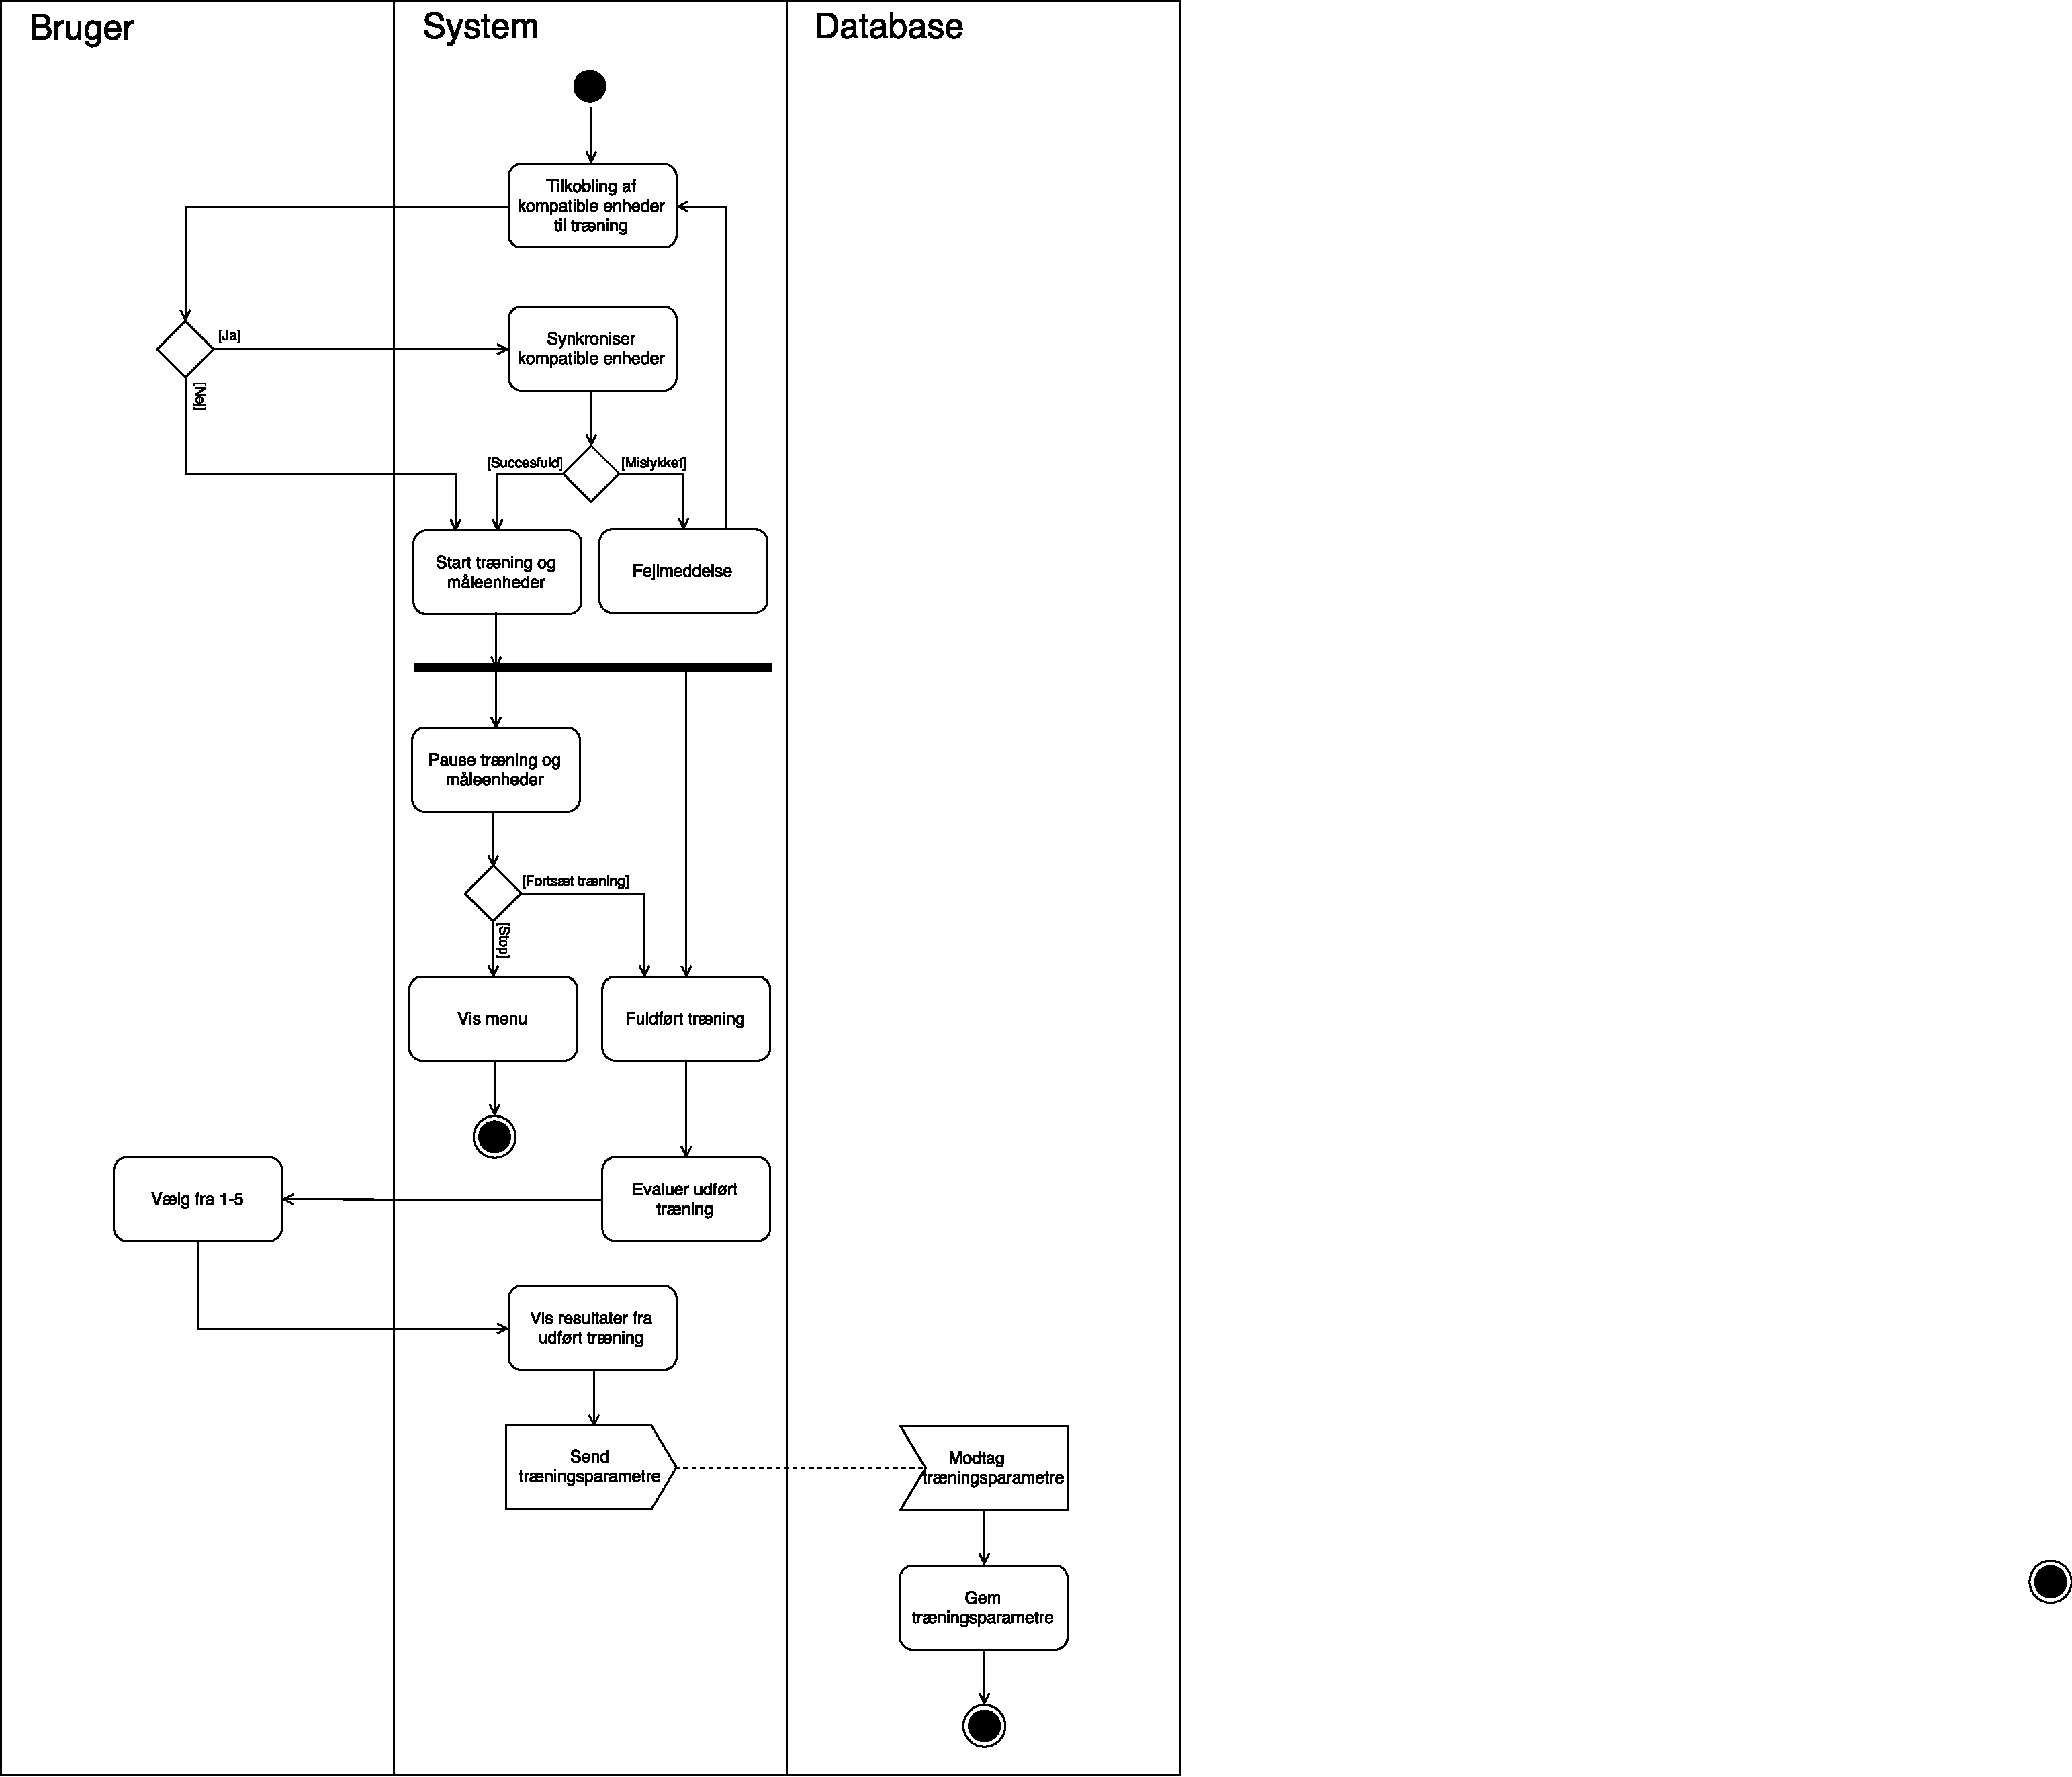
\includegraphics[width=1\textwidth]{figures/aktivitetsdiagram/Traening}
\caption{Aktivitetsdiagram over træning.}
\label{fig:traening}
\end{figure}

\noindent
Når systemet har tilpasset træningniveau, vises grænsefladen for træning. Brugeren kan påbegynde træningen ved at trykke start, hvorefter timer og GPS starter. Under træningen vil tid og afstand kontinuert fremgå af grænsefladen. Brugeren kan til en hver tid vælge at afslutte træningen ved at trykke på stop, hvilket medfører, at timer og GPS stoppes og grænsefladen for afslut træning vises. Denne handling skal bekræftes i tilfælde af, at brugeren ved en fejl angiver, at træningen skal stoppes. Er dette tilfældet afsluttes træningen ikke og grænsefladen for træning vises igen. Ved bekræftelse af stop træning, vises grænsefladen for evaluering af udført træning, hvor brugeren skal angive en evaluering. Efterfølgende sendes evalueringen og træningsresultater til databasen, hvor det gemmes.

